\documentclass[10pt]{beamer}
%Available font sizes are 8pt, 9pt, 10pt, 11pt, 12pt, 14pt, 17pt, 20pt. Default font size is 11pt

%%%%%%%%%%%%%%%%%%%%%%%%%%%%%% beamer直接在设置超链接 %%%%%%%%%%%%

\hypersetup{colorlinks=true,allcolors=.,citecolor = magenta,anchorcolor=red,urlcolor=blue!60!black}

%\hypersetup{
%%	colorlinks=true,citecolor = green,urlcolor=blue,
%%	urlcolor=blue,
%%	urlbordercolor=blue,
%	pdfborder={1 1 1},
%	pdfborderstyle={/S/U/W 1}   
%}

% 控制下划线包
%\usepackage{ulem}

%\usetheme{Madrid}
%\usetheme{Berkeley}
%\usetheme{Copenhagen}
%\usepackage{lineno,hyperref}
\usepackage[utf8]{inputenc}
\usetheme[]{Berlin} %T
%\usetheme{Boadilla} %T
%\usetheme{Darmstadt} %T
%\usetheme{Frankfurt} %T
%\usetheme{Ilmenau}
%\usetheme{Dresden}

%\usetheme{Boadilla}
%\usetheme{CambridgeUs}
%\usetheme{Copenhagen}
%\usetheme{Warsaw}

%\usecolortheme{default}
\usecolortheme{beaver}
%\usecolortheme{seahorse}
%\usecolortheme{wolverine}
%\usecolortheme{beetle}


%%%%%%%%%%%%%%%%%%%%%%%%%%%%% 设置标题阴影 %%%%%%%%%%%%%%%%%%%%%
\setbeamertemplate{title page}[default][colsep=-4bp,rounded=true,shadow=true]


% ################################ 设置页眉 ##########################
% 去掉 子标题subsection
\defbeamertemplate*{headline}{miniframes theme no subsection}
{%
	\begin{beamercolorbox}[colsep=1.5pt]{upper separation line head}
	\end{beamercolorbox}
	\begin{beamercolorbox}{section in head/foot}
		\vskip2pt\insertnavigation{\paperwidth}\vskip2pt
	\end{beamercolorbox}%
	\begin{beamercolorbox}[colsep=1.5pt]{lower separation line head}
	\end{beamercolorbox}
}

\setbeamertemplate{footline}[miniframes theme no subsection]



%%%%%%%%%%%%%%%%%%%%%%%%%%%%%%%%%%% 设置页脚 %%%%%%%%%%%%%%%%%%%%%%%%%%%%%%

\makeatletter
\defbeamertemplate*{footline}{myfootline}
{
	\leavevmode%
	\hbox{%
		\begin{beamercolorbox}[wd=.4\paperwidth,ht=2.5ex,dp=1ex,center]{title in head/foot}%
			\usebeamerfont{title in head/foot}\insertshorttitle
		\end{beamercolorbox}%
		\begin{beamercolorbox}[wd=.2\paperwidth,ht=2.5ex,dp=1ex,center]{title in head/foot}%
			\usebeamerfont{author in head/foot}\insertshortauthor\expandafter\beamer@ifempty\expandafter{\beamer@shortinstitute}{}{~~\insertshortinstitute}
		\end{beamercolorbox}%
		\begin{beamercolorbox}[wd=.4\paperwidth,ht=2.5ex,dp=1ex,right]{title in head/foot}%
			\usebeamerfont{date in head/foot}\insertshortdate{}\hspace*{2em}
			\insertframenumber{} / \inserttotalframenumber\hspace*{2ex} 
	\end{beamercolorbox}}%
	\vskip0pt%
}
\makeatother
\setbeamertemplate{footline}[myfootline]
%%%%%%%%%%%%%%%%%%%%%%%%%%%%%%%%%%%%%%%%%%%%%%%%%%%%%%%%%%%%%%%%%%%%%%%%%%%

% ############################## 图片 ######################
\usepackage{graphicx}
\usepackage{subfigure}
\setbeamertemplate{caption}[numbered]

\usepackage{pgfplots}
\usepackage{pgfplotstable}
\pgfplotsset{width=7cm,compat=1.17}

% ############################################

% ################# 项目符号 ###############
\usepackage{tikz}
\setbeamertemplate{items}[ball]
\setbeamercolor{itemize item}{fg=red}

% #########################################

% 字体
\usepackage{fontspec}
\setmainfont{Times New Roman}
%structurebold, structurebolditalic, structuresmallcapsserif, structureitalicsserif, serif and default.
\usefonttheme{serif}

%字体类型 mathptmx, helvet, avat, bookman, chancery, charter, culer, mathtime, mathptm, newcent, palatino, and pifont.
%\usepackage{helvet}

%去掉右下角按钮
\setbeamertemplate{navigation symbols}{}


%%%%%%%%%%%%%%%%%%%%%%%%%%%%%%%%%%%%%%%%%% 参考文献 %%%%%%%%%%%%%%%%%%%%%
%设置参考文献布局格式,去掉beamer默认的符号
%\usepackage{cite}
%\bibliographystyle{plain}
% style和citestyle参数分别是参考文献排列格式和引用格式
% style 常见有numeric authoryear authoryear-icomp apa
% citestyle常见有APA 
% \textcite 引用为author (year) \parencite 格式为(author,year;author,year)
\usepackage[backend=biber, style=apa, citestyle=APA, sorting=anyt]{biblatex}
\addbibresource{preRefs.bib}

\setbeamertemplate{bibliography item}[triangle]

\AtBeginBibliography{\footnotesize}

% \textcite{} 命令配置
\DeclareCiteCommand{\textcite}
{\boolfalse{cbx:parens}}
{\usebibmacro{citeindex}%
	\printtext[bibhyperref]{\printnames{labelname}%
		\printtext{ (\printfield{year}\printtext{)}}}}
{\ifbool{cbx:parens}
	{\bibcloseparen\global\boolfalse{cbx:parens}}
	{}%
	\multicitedelim}
{\usebibmacro{textcite:postnote}}

% \parencite{} 命令配置
%\DeclareCiteCommand{\parencite}
%{\boolfalse{cbx:parens}}
%{\usebibmacro{citeindex}%
%	\printtext[bibhyperref]{(\printnames{labelname}%
%		\printtext, { \printfield{year}\printtext)}}}
%{\ifbool{cbx:parens}
%	{\bibcloseparen\global\boolfalse{cbx:parens}}
%	{}%
%	\multicitedelim}
%{\usebibmacro{parencite:postnote}}

%%%%%%%%%%%%%%%%%%%%%%%%%%%%%%%%%%%%%%%%%% 参考文献 %%%%%%%%%%%%%%%%%%%%%
%\date{\today}
%\author{LEI LI}
%\institute[UCAS]{University of Chinese Academy of Science}

\title{Artificial Intelligence Application in Finance and Economics}
\subtitle{State of the art}

\author[Arthur, Doe] % (optional)
{A.~B.~Arthur\inst{1} \and J.~Doe\inst{2}}

\institute[VFU] % (optional)
{
	\inst{1}%
	Faculty of Physics\\
	Very Famous University
	\and
	\inst{2}%
	Faculty of Chemistry\\
	Very Famous University
}

%\date[VLC 2021] % (optional)
%{Very Large Conference, April 2021}

\date{\today}
%\logo{
%	\begin{tikzpicture}
%		\filldraw[color=red!50, fill=red!25, very thick](0,0) circle (0.5);
%		\node[draw,color=white] at (0,0) {a};
%	\end{tikzpicture}}


%%%%%%%%%%%%%%%%%%%%%%%%%%% 设置ppt背景 %%%%%%%%%%%%%%%%%%%%%%
\newcommand\Background{%
	\begin{tikzpicture}[remember picture,overlay]
		\node[inner sep=0pt,outer sep=0pt,opacity=0.1]
		at (current page.center)
		{\includegraphics[scale=0.2]{img/bg}};
	\end{tikzpicture}
}
%%%%%%%%%%%%%%%%%%%%%%%%%%%%%%%%%%%%%%%%%%%%%%%%%%%%%%%%%%%%


\AtBeginSection[]
{
	\begin{frame}
		\frametitle{Outline}
		\tableofcontents[currentsection]
	\end{frame}
}

\begin{document}
	\begin{frame}
%		\Background
		\titlepage
	\end{frame}

	\begin{frame}
		\frametitle{Outline}
		\tableofcontents
	\end{frame}

	\section{Introduction}
%	\subsection{AAAA}
	\begin{frame}{Introduction}
		%方框
		\begin{definition}
			\small {A \alert{prime number} is a number that has exactly two.}
		\end{definition}
		
		\begin{example}
			\begin{itemize}
				\small{
				\item 2 is prime (two divisors: 1 and 2).
				\item 3 is prime (two divisors: 1 and 3).
				\item 4 is not prime (\alert{three} divisors: 1, 2, and 4).}
			\end{itemize}
		\end{example}
		%enumrate无序列表
		\begin{itemize}
%			\setbeamertemplate{itemize items}{\color{red}$\bullet$}
			\setbeamertemplate{itemize items}[ball]
			
			\item {\small \bf LATEX normally chooses the appropriate font and font size based on the logical structure of the document (e.g. sections). In some cases, you may want to set fonts and sizes by hand!}
			\item[-]<1-> Text visible on slide 1
			\item[$\circ$]<2-> Text visible on slide 2
			\item<3> Text visible on slides 3
			\item<4-> Text visible on slide 4
		\end{itemize}
	\end{frame}
	\begin{frame}{Second Frame}
%		\framesubtitle{SSSSSS}
%		\begin{theorem}
%			There is no largest prime number.
%		\end{theorem}
		\begin{proof}
			%enumrate有序列表
			\begin{enumerate}
				\item<1-> Suppose $p$ were the largest prime number.
				\item<2-> Let $q$ be the product of the first $p$ numbers.
				\item<3-> Then $q + 1$ is not divisible by any of them.
				\item<1-> But $q + 1$ is greater than $1$, thus divisible by some prime number not in the first $p$ numbers.\qedhere
			\end{enumerate}
		\end{proof}
		\uncover<4->{The proof used \textit{reductio ad absurdum}.}
		\begin{itemize}
			\item 2 is prime (two divisors:1 and 2).
			\pause
			\item 3 is prime (two divisors:1 and 3).
			\pause
			\item 4 is prime (two divisors:1 and 2,4).
		\end{itemize}
	\end{frame}
	
	\section{Literature Reviews}
	\begin{frame}
		\frametitle{Literature Reviews}
		\begin{block}{Answered Questions}
			How many primes are there?\textcite{deng2014deep}
		\end{block}
		\begin{block}{Open Questions}
			Is every even number the sum of two primes?\parencite{mackenzie1992risk}
		\end{block}
	\end{frame}
	
	\section{Methods}
	\begin{frame}
		\frametitle{Sample frame title}
		
		In this slide, some important text will be
		\alert{highlighted} because it's important.
		Please, don't abuse it.
		
		\begin{block}{Remark}
			Sample text
		\end{block}
		
		\begin{alertblock}{Important theorem}
			Sample text in red box
		\end{alertblock}
		
		\begin{examples}
			Sample text in green box. The title of the block is ``Examples".
		\end{examples}
	\end{frame}
	\begin{frame}
		\frametitle{Two-column slide}
		\begin{columns}
			\column{0.5\textwidth}
			This is a text in first column.
			$$E=mc^2$$
			\begin{itemize}
				\item First item
				\item Second item
			\end{itemize}
			
			\column{0.5\textwidth}
			{\small \textcite{kamilaris2018deep} will be in the second column(Fig. \ref{g2})
			and on a second thoughts\parencite{deng2014deep}, this is a nice looking
			layout in some cases\parencite{deng2014deep,kamilaris2018deep,mackenzie1992risk}.}
		\end{columns}
	\end{frame}
	\begin{frame}
		\frametitle{Graph}
		\begin{itemize}
			\item Beijing
			\item Shanghai
			\item Shenzhen
		\end{itemize}
		\begin{figure}[]
			\centering
			
\includegraphics[scale=0.4]{img/g1}
			\caption{Artificial Intelligence}
		\end{figure}
	\end{frame}
	\begin{frame}
		\frametitle{Com-Graph-1}
		\begin{figure}
			\centering
			\subfigure[AI-N]{
\includegraphics[width=2.5cm,height=2cm]{img/g2}\label{g2}}
			\subfigure[AI-M]{
\includegraphics[width=2.5cm,height=2cm]{img/g3}\label{g3}}
			\subfigure[AI-M]{
\includegraphics[width=2.5cm,height=2cm]{img/g4}\label{g4}}
			\subfigure[AI-M]{
\includegraphics[width=2.5cm,height=2cm]{img/g5}\label{g5}}
			\caption{AI-COM}
		\end{figure}
	\end{frame}

	\begin{frame}
		\frametitle{Com-Graph-2}
		\begin{columns}
			\column{0.4\textwidth}
			\begin{itemize}
				\item[$\circledcirc$] This code will generate three slides to add a visual effect to the presentation. will prevent the text below this point and above the next declaration to appear in the current slide.
			\end{itemize}
			
			\column[]{0.6\textwidth}
			\begin{figure}
				\centering
				\subfigure[AI-N]{
\includegraphics[width=3cm,height=2.2cm]{img/g2}\label{g2}}
				\subfigure[AI-M]{
\includegraphics[width=3cm,height=2.2cm]{img/g3}\label{g3}}\\
				\subfigure[AI-M]{
\includegraphics[width=3cm,height=2.2cm]{img/g4}\label{g4}}
				\subfigure[AI-M]{
\includegraphics[width=3cm,height=2.2cm]{img/g5}\label{g5}}
				\caption{AI-COM}
			\end{figure}
		\end{columns}
	\end{frame}

	\begin{frame}
		\frametitle{Com-Graph-3}
		\begin{columns}
			\column{0.6\textwidth}
			\begin{itemize}
				\item[$\bigstar$] This code will generate three slides to add a visual effect to the presentation..
				\item[$\blacktriangleright$] This code will generate three slides to add a visual effect to the presentation.
				\item[$\divideontimes$] aaaaaaaaa
				\item[$\checkmark$] AAAAAAAAA...
				\item[$\circledcirc$] AAAAAAAAA...
				\item[$\circleddash$] AAAAAAAAA...
				\item[$\bigodot$] BBBB...
				\item[$\boxdot$] BBBB...
				\item[$\nabla$] BBBB...
				\item[$\Delta$] BBBB...
			\end{itemize}
			
			\column[]{0.4\textwidth}
			\begin{figure}
				\centering
				\subfigure[AI-N]{
\includegraphics[width=3cm,height=2.2cm]{img/g2}\label{g6}} \\
				\subfigure[AI-M]{
\includegraphics[width=3cm,height=2.2cm]{img/g3}\label{g7}}
				\caption{AI-MN}
			\end{figure}
		\end{columns}
	\end{frame}

	\begin{frame}
		\frametitle{Com-Graph-4}
		\begin{columns}
			\column{0.4\textwidth}
			\begin{itemize}
				\item[$\circledcirc$] This code will generate three slides to add a visual effect to the presentation. will prevent the text below this point and above the next declaration to appear in the current slide.
			\end{itemize}
			
			\column[]{0.6\textwidth}
			\begin{figure}
				\centering
				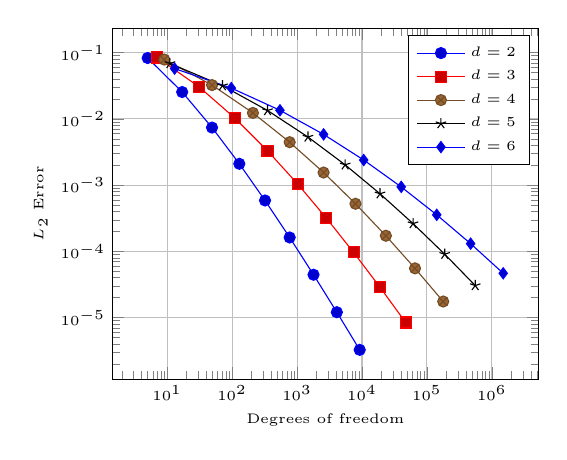
\begin{tikzpicture}
					\begin{loglogaxis}[
						xlabel={Degrees of freedom},
						ylabel={$L_2$ Error},
						grid = major
						]
						\addplot coordinates {
							(5,8.312e-02)    (17,2.547e-02)   (49,7.407e-03)
							(129,2.102e-03)  (321,5.874e-04)  (769,1.623e-04)
							(1793,4.442e-05) (4097,1.207e-05) (9217,3.261e-06)
						};
						
						\addplot coordinates{
							(7,8.472e-02)    (31,3.044e-02)    (111,1.022e-02)
							(351,3.303e-03)  (1023,1.039e-03)  (2815,3.196e-04)
							(7423,9.658e-05) (18943,2.873e-05) (47103,8.437e-06)
						};
						
						\addplot coordinates{
							(9,7.881e-02)     (49,3.243e-02)    (209,1.232e-02)
							(769,4.454e-03)   (2561,1.551e-03)  (7937,5.236e-04)
							(23297,1.723e-04) (65537,5.545e-05) (178177,1.751e-05)
						};
						
						\addplot coordinates{
							(11,6.887e-02)    (71,3.177e-02)     (351,1.341e-02)
							(1471,5.334e-03)  (5503,2.027e-03)   (18943,7.415e-04)
							(61183,2.628e-04) (187903,9.063e-05) (553983,3.053e-05)
						};
						
						\addplot coordinates{
							(13,5.755e-02)     (97,2.925e-02)     (545,1.351e-02)
							(2561,5.842e-03)   (10625,2.397e-03)  (40193,9.414e-04)
							(141569,3.564e-04) (471041,1.308e-04) (1496065,4.670e-05)
						};
						\tiny\legend{$d=2$,$d=3$,$d=4$,$d=5$,$d=6$}
					\end{loglogaxis}
				\end{tikzpicture}
				\caption{Results of Experiment}
			\end{figure}
			
%			\begin{tikzpicture}
%				\begin{axis}[
%					ybar,
%					enlargelimits=0.15,
%					legend style={at={(0.5,-0.15)},
%						anchor=north,legend columns=-1},
%					ylabel={\#participants},
%					symbolic x coords={tool8,tool9,tool10},
%					xtick=data,
%					nodes near coords,
%					nodes near coords align={vertical},
%					]
%					\addplot coordinates {(tool8,7) (tool9,9) (tool10,4)};
%					\addplot coordinates {(tool8,4) (tool9,4) (tool10,4)};
%					\addplot coordinates {(tool8,1) (tool9,1) (tool10,1)};
%					\legend{used,understood,not understood}
%				\end{axis}
%			\end{tikzpicture}
		\end{columns}
	\end{frame}
	\begin{frame}
		\begin{itemize}
			\item[$\Delta$]Exprimental Result about DPN
		\end{itemize}
		 
		\begin{figure}
			\pgfplotsset{width = 5.5cm,height=4.5cm,
				tick label style={font=\footnotesize},
				label style={font=\footnotesize},
				legend style={font=\footnotesize},}
			\subfigure[R1]{
				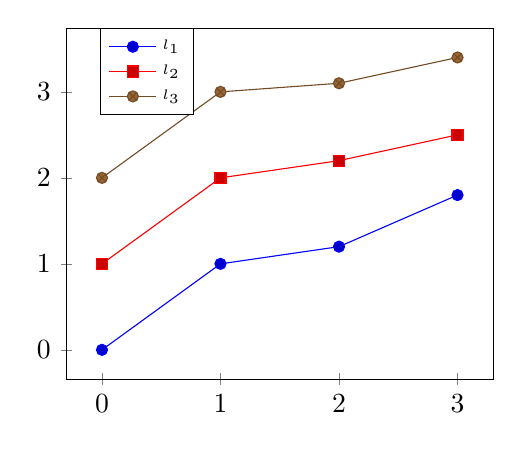
\begin{tikzpicture}
					\begin{axis}[
						% this modifies 'every axis legend':
						legend style={at={(0.3,1)},font=\tiny,},
						xtick pos=lower,
						ytick pos=left, 
						xtick align=center,
						ytick align=center]
						\addplot coordinates {(0,0) (1,1) (2,1.2) (3,1.8)};						
						\addplot coordinates {(0,1) (1,2) (2,2.2
							) (3,2.5)};
						\addplot coordinates {(0,2) (1,3) (2,3.1) (3,3.4)};
						\legend{$l_1$,$l_2$,$l_3$}
					\end{axis}
				\end{tikzpicture}
			}
			\subfigure[R2]{
				 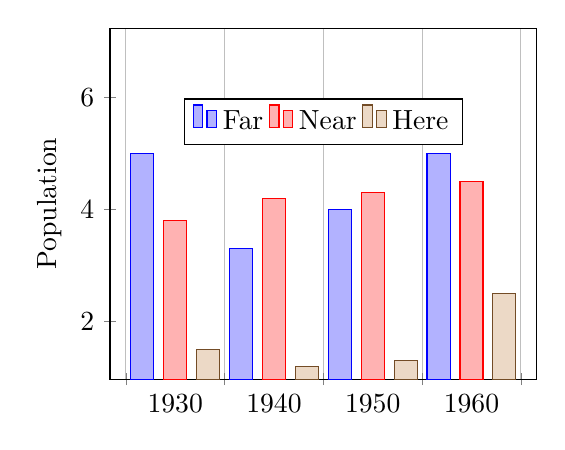
\begin{tikzpicture}
					\begin{axis}[
						x tick label style={
							/pgf/number format/1000 sep=},
						ylabel=Population,
						enlargelimits=0.04,
						legend style={at={(0.5,0.8)},
							anchor=north,legend columns=-1},
						ybar interval=0.7,
						xtick pos=lower,
						ytick pos=left,
						xtick align=center,
						ytick align=center
						]
						\addplot 
						coordinates {(1930,5) (1940,3.3)
							(1950,4) (1960,5) (1970,7)};
						
						\addplot 
						coordinates {(1930,3.8) (1940,4.2) 
							(1950,4.3) (1960,4.5) (1970,6.5)};
						
						\addplot 
						coordinates {(1930,1.5) (1940,1.2) 
							(1950,1.3) (1960,2.5) (1970,3.5)};
						\legend{Far,Near,Here}
					\end{axis}
				\end{tikzpicture}
			}
		\caption{Results of Exp}
		\end{figure}
			
	\end{frame}

	\section{Conclusions}
	\begin{frame}
		AAAAAA  {\color{red} \url{http://www.baidu.com}}\\
		{\color{red}\underline{\href[]{http://www.overleaf.com}{Something 
					Linky}}} \\
		
%		\href{http://url.com}{displayed, underlined text}
	\end{frame}

%	\newpage
%	有很多参考文献需要换页时候可加上[allowframebreaks]参数
%	\section{References}
	\begin{frame}{References}
%		\footnotesize\bibliography{preRefs}
		\printbibliography
%		\printbibliography[heading=bibintoc,title={Whole bibliography}]
	\end{frame}
	\begin{frame}
		\centering \Large{Thank you for listening!}
	\end{frame}

\end{document}